\chapter{Aplicaciones del código de simulación}
\label{aplicaciones}

\section{Aplicación para el análisis paramétrico}
\label{analisis-parametrico}

Una vez que hemos confirmado que nuestro código es una herramienta válida para la simulación de un campo solar real, nos proponemos, a continuación, aprovecharlo para analizar el comportamiento de los componentes del campo solar bajo diferentes condiciones o con diferentes configuraciones. Este tipo de análisis es de especial utilidad durante la fase de diseño, cuando deben seleccionarse los componentes del sistema con el fin de alcanzar unos objetivos de rendimiento o potencia generada.

\subsection{Rendimiento del HCE en función de la radiación normal directa, $DNI$}

En la tabla \ref{tab:datos_hces} se muestran los coeficientes para el cálculo de la emisividad $\varepsilon_{ext}$ conforme a la ec.\eqref{eq:eext} y el valor de la absortividad de algunos modelos de HCE según se recogen en \cite{barberofresnoDesarrolloModeloTeorico2018}, incluido el modelo NREL\#6, que en realidad es un modelo de HCE con un recubrimiento selectivo teórico propuesto para desarrollos futuros.

\begin{longtable}[c]{lccc}
\caption[Constantes del modelo de emisividad equivalente para cada uno de los receptores seleccionados]{Constantes del modelo de emisividad equivalente para cada uno de los receptores seleccionados.}
\label{tab:datos_hces}  \\ \hline
Receptor &
$A_0$ &
$A_1$ &
Absortividad (\%) \\ \hline
Solel UVAC 2/2008 & 1,31E-04 & 1,01E-01 & 97\\
Solel UVAC 3/2010 & 2,06E-04 & 4,30E-02 & 96 \\
Schott PTR70 & 1,82E-04 & 8,61E-02 & 95 \\
Schott PTR70/2008 & 1,43E-04 & 3,45E-02 & 95,5 \\
SkyFuel SkyTrough DSP & 1,48E-04 & 4,00E-02 & 95 \footnote{Al no disponerse de este dato, se ha empleado este valor con el fin de poder incluir el modelo en el test. Fuente \cite{barberofresnoDesarrolloModeloTeorico2018}}\\
ASE HEMS08 & 2,03E-04 & -1,03E-02 & 95 \\
NREL \#6 & 1,52E-04 & 1,96E-03 & 96 
\end{longtable}



Si simulamos el comportamiento de un único HCE de cada modelo (considerando que todos tienen la misma longitud de 4,05 m),  para  diferentes valores de DNI y bajo las mismas condiciones de caudal y temperatura de entrada del HTF, podemos realizar una comparativa de los rendimientos. Salvo que se diga lo contrario, en adelante emplearemos los mismos datos geográficos ya indicados cuando realizamos la simulación de verificación con SAM. Para la fecha y hora de simulación se empleará el 1 de julio a las 12:00 UTC (14:00 hora local).

A modo de ejemplo, se muestra el código  \ref{lst:script_test1} desarrollado para realizar este tipo de simulación a partir de un archivo de configuración \emph{test\_1.json}.  Este archivo es similar al mostrado en el apartado anterior, con las siguientes salvedades:
\begin{itemize}
\item
Solo es necesasrio indicar la configuración de un solo lazo con un único SCA que contiene un único HCE. De este modo, simulamos solo un HCE de 4,05 m.
\item 
El archivo de origen de datos contiene varios registros con los mismos datos de fecha, hora, temperatura ambiente y viento, pero varía la DNI desde 100 hasta 1000 $W/m^2$.
\end{itemize}

El programa se dispone a hacer una simulación con la configuración indicada para cada registro del archivo de origen de datos, pero también realiza un bucle recorriendo todos los modelos de HCE que existen en el archivo \emph{HCE\_library.json}. De esta forma, al finalizar, tenemos una tabla con el rendimiento de cada modelo para cada uno de los valores de DNI. Se hace uso de la Clase \texttt{LoopSimulation} creada expresamente con el fin de facilitar simulaciones con un solo lazo de configuración variable.

\begin{lstlisting}[caption=Programa para el análisis del rendimiento en función de DNI, label={lst:script_test1}]
import csenergy as cs
import pandas as pd
import json
from datetime import datetime

FLAG_00 = datetime.now()
with open("./saved_configurations/test_1.json") as simulation_file:
    simulation_settings = json.load(simulation_file)
with open("./hce_files/HCE_library.json") as hces_file:
    hces_configurations = json.load(hces_file)
dict_resultados = {}
for hce_conf in hces_configurations:
    simulation_settings['HCE'].update(hce_conf)
    dni_index = []
    simulation = cs.LoopSimulation(simulation_settings)
    dict_resultados[hce_conf['Name']] = []
    for row in simulation.datasource.dataframe.iterrows():
        solarpos = simulation.site.get_solarposition(row)
        aoi = simulation.base_loop.scas[0].get_aoi(solarpos)
        values = {'tin': 573,
                  'pin': 1900000,
                  'massflow': 6}
        simulation.base_loop.initialize('values', values)
        simulation.base_loop.calc_loop_pr_for_massflow(
            row,
            solarpos,
            simulation.htf,
            simulation.model)
        tout = simulation.base_loop.scas[-1].hces[-1].tout
        pout = simulation.base_loop.scas[-1].hces[-1].pout
        simulation.base_loop.set_loop_values_from_HCEs()
        pr = simulation.base_loop.pr
        dict_resultados[hce_conf['Name']].append(pr)
        dni_index.append(row[1]['DNI'])
        simulation.datasource.dataframe.at[row[0], 'pr'] = pr
        simulation.datasource.dataframe.at[row[0], 'tout'] = tout
        simulation.datasource.dataframe.at[row[0], 'pout'] = pout
dfsalida = pd.DataFrame(dict_resultados, index=dni_index)
dfsalida.to_csv('rendimiento_dni.csv', sep=';', decimal=',')
FLAG_01 = datetime.now()
DELTA_01 = FLAG_01 - FLAG_00
print("Total runtime: ", DELTA_01.total_seconds())
\end{lstlisting}

El tiempo total de ejecución es de 1,375 segundos. El archivo \emph{rendimiento\_dni.csv} contiene los datos volcados a la finalización del programa.

En la tabla \ref{tab:rendimiento_hce_dni} se muestran los resultados de los rendimientos calculados para cada modelo de HCE con una temperatura de entrada de 300 ºC y un caudal de 6 kg/s.

\begin{longtable}[c]{cccccccc}
\caption{Rendimiento en función de la radiación normal incidente para  distintos modelos de HCE}
\label{tab:rendimiento_hce_dni} \\ \hline
\parbox{3em}{\centering \rule{0pt}{2ex} DNI \\ $(W/m^2)$} &
\parbox{3em}{\centering \rule{0pt}{2ex} Schott  \\ PTR70} &
\parbox{3em}{\centering \rule{0pt}{2ex} Schott  \\ PTR70 2008} &
\parbox{3em}{\centering \rule{0pt}{2ex} Solel \\ UVAC 2} &
\parbox{3em}{\centering \rule{0pt}{2ex} Solel \\ UVAC 3} &
\parbox{4em}{\centering \rule{0pt}{2ex} SkyFuel \\ SkyTrough DSP} &
\parbox{3em}{\centering \rule{0pt}{2ex} ASE\\ HEMS08} &
\parbox{3em}{\centering \rule{0pt}{2ex} NREL\\ \#6} \\ \hline
100 & 0,521 & 0,728 & 0,521 & 0,638 & 0,837 & 0,818 & 0,834 \\
200 & 0,757 & 0,862 & 0,757 & 0,816 & 0,917 & 0,907 & 0,916 \\
300 & 0,837 & 0,907 & 0,837 & 0,876 & 0,944 & 0,938 & 0,943 \\
400 & 0,876 & 0,930 & 0,877 & 0,907 & 0,958 & 0,953 & 0,957 \\
500 & 0,900 & 0,944 & 0,900 & 0,925 & 0,966 & 0,962 & 0,965 \\
600 & 0,917 & 0,953 & 0,917 & 0,937 & 0,971 & 0,968 & 0,971 \\
700 & 0,928 & 0,959 & 0,928 & 0,945 & 0,975 & 0,972 & 0,975 \\
800 & 0,937 & 0,964 & 0,937 & 0,952 & 0,978 & 0,976 & 0,978 \\
900 & 0,943 & 0,968 & 0,943 & 0,957 & 0,980 & 0,978 & 0,980 \\
1000 & 0,948 & 0,971 & 0,949 & 0,961 & 0,982 & 0,980 & 0,982
\end{longtable}

En la Fig.\ref{fig:test1a} se muestra gráficamente cómo evoluciona el rendimiento con el aumento de $DNI$.  Se aprecia cómo los  modelos de última generación presentan un buen comportamiento incluso con bajas radiaciones.

\begin{figure}[H]
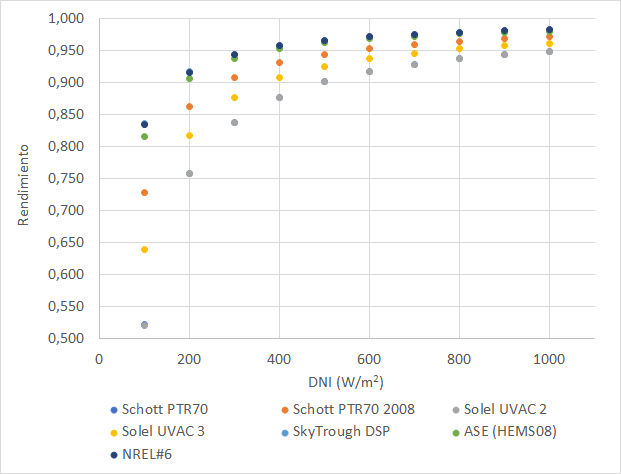
\includegraphics[width=0.8\linewidth, height=0.55\linewidth]{images/rendimiento_dni.png}
\caption[Rendimiento térmico en función de DNI para diferentes modelos de HCE]{Rendimiento térmico en función de DNI para diferentes modelos de HCE. $T_{in}$=300 ºC, $\dot m$ = 6 kg/s} 
\label{fig:test1a}
\end{figure}


\subsection{Rendimiento del HCE en función de la temperatura de entrada}

Otra decisión importante que debe tomarse a la hora del diseño de  un campo solar es la temperatura nominal de operación. Intervienen varios criterios, como la temperatura y el caudal de fluido caloportador que demanda el bloque de potencia así como las limitaciones que impone el propio fluido a fin de evitar su degradación.  Un análisis del rendimiento del HCE en función de la temperatura de operación puede ayudar en la toma de decisiones y  en la selección del modelo más adecuado.

El procedimiento es muy parecido al caso anterior tal y como se muestra en el \ref{lst:script_test2}, que mostramos a continuación a modo de ejemplo\footnote{El resto de \emph{scripts} para los diferentes test realizados en este capítulo pueden encontrarse el el archivo que contiene la versión electrónica de este TFG}, solo que en esta ocasión lo que se hace es ir modificando la temperatura de entrada. 

\begin{lstlisting}[caption=Programa para el análisis del rendimiento en función de $T_{in}$, label={lst:script_test2}]
with open("./saved_configurations/test_2.json") as simulation_file:
    simulation_settings = json.load(simulation_file)
with open("./hce_files/HCE_library.json") as hces_file:
    hces_configurations = json.load(hces_file)
dict_resultados = {}
for hce_conf in hces_configurations:
    simulation_settings['HCE'].update(hce_conf)
    tin_index = []
    simulation = cs.LoopSimulation(simulation_settings)
    dict_resultados[hce_conf['Name']] = []
    for row in simulation.datasource.dataframe.iterrows():
        solarpos = simulation.site.get_solarposition(row)
        aoi = simulation.base_loop.scas[0].get_aoi(solarpos)
        for tin in range(473, 693, 10):
            values = {'tin': tin,
                      'pin': 1900000,
                      'massflow': 6}
            simulation.base_loop.initialize('values', values)
            simulation.base_loop.calc_loop_pr_for_massflow(
                row,
                solarpos,
                simulation.htf,
                simulation.model)
            tout = simulation.base_loop.scas[-1].hces[-1].tout
            pout = simulation.base_loop.scas[-1].hces[-1].pout
            simulation.base_loop.set_loop_values_from_HCEs()
            pr = simulation.base_loop.pr
            dict_resultados[hce_conf['Name']].append(pr)
            tin_index.append(tin-273)
            simulation.datasource.dataframe.at[row[0], 'pr'] = pr
            simulation.datasource.dataframe.at[row[0], 'tout'] = tout
            simulation.datasource.dataframe.at[row[0], 'pout'] = pout
dfsalida = pd.DataFrame(dict_resultados, index=tin_index)
print(dfsalida)
dfsalida.to_csv('rendimiento_temperatura.csv', sep=';', decimal=',')
\end{lstlisting}

En la tabla \ref{tab:rendimiento_hce_tin} se muestran los resultado de simular el funcionamiento de varios modelos de HCE con un caudal constante de fluido caloportador a diferentes temperaturas de entrada.

\begin{longtable}[c]{cccccccc}
\caption{Rendimiento en función de la temperatura de entrada del HTF para diferentes modelos de HCE}
\label{tab:rendimiento_hce_tin} \\ \hline
\parbox{3em}{\centering \rule{0pt}{2ex} $T_{in} (\circ C)$ } &
\parbox{3em}{\centering \rule{0pt}{2ex} Schott  \\ PTR70} &
\parbox{3em}{\centering \rule{0pt}{2ex} Schott  \\ PTR70 2008} &
\parbox{3em}{\centering \rule{0pt}{2ex} Solel \\ UVAC 2} &
\parbox{3em}{\centering \rule{0pt}{2ex} Solel \\ UVAC 3} &
\parbox{4em}{\centering \rule{0pt}{2ex} SkyFuel \\ SkyTrough DSP} &
\parbox{3em}{\centering \rule{0pt}{2ex} ASE\\ HEMS08} &
\parbox{3em}{\centering \rule{0pt}{2ex} NREL\\ \#6} \\ \hline
\endfirsthead
\multicolumn{4}{c}%
{{Tabla \thetable\ continúa desde la página anterior}} \\ \hline
\parbox{3em}{\centering \rule{0pt}{2ex} $T_{in} (\circ C)$ } &
\parbox{3em}{\centering \rule{0pt}{2ex} Schott  \\ PTR70} &
\parbox{3em}{\centering \rule{0pt}{2ex} Schott  \\ PTR70 2008} &
\parbox{3em}{\centering \rule{0pt}{2ex} Solel \\ UVAC 2} &
\parbox{3em}{\centering \rule{0pt}{2ex} Solel \\ UVAC 3} &
\parbox{4em}{\centering \rule{0pt}{2ex} SkyFuel \\ SkyTrough DSP} &
\parbox{3em}{\centering \rule{0pt}{2ex} ASE\\ HEMS08} &
\parbox{3em}{\centering \rule{0pt}{2ex} NREL\\ \#6} \\ \hline
\endhead
200 & 0,975 & 0,986 & 0,974 & 0,982 & 0,993 & 0,993 & 0,993 \\
210 & 0,972 & 0,985 & 0,971 & 0,980 & 0,992 & 0,992 & 0,992 \\
220 & 0,969 & 0,983 & 0,969 & 0,978 & 0,991 & 0,990 & 0,991 \\
230 & 0,966 & 0,981 & 0,965 & 0,976 & 0,990 & 0,989 & 0,990 \\
240 & 0,963 & 0,979 & 0,962 & 0,973 & 0,988 & 0,988 & 0,988 \\
250 & 0,959 & 0,977 & 0,958 & 0,970 & 0,987 & 0,986 & 0,987 \\
260 & 0,955 & 0,975 & 0,955 & 0,967 & 0,986 & 0,984 & 0,985 \\
270 & 0,951 & 0,973 & 0,951 & 0,964 & 0,984 & 0,982 & 0,984 \\
280 & 0,946 & 0,970 & 0,946 & 0,960 & 0,982 & 0,980 & 0,982 \\
290 & 0,942 & 0,967 & 0,942 & 0,956 & 0,980 & 0,978 & 0,980 \\
300 & 0,937 & 0,964 & 0,937 & 0,952 & 0,978 & 0,976 & 0,978 \\
310 & 0,931 & 0,961 & 0,931 & 0,947 & 0,976 & 0,973 & 0,975 \\
320 & 0,925 & 0,957 & 0,926 & 0,943 & 0,974 & 0,970 & 0,973 \\
330 & 0,919 & 0,953 & 0,920 & 0,938 & 0,971 & 0,967 & 0,970 \\
340 & 0,912 & 0,949 & 0,914 & 0,932 & 0,968 & 0,963 & 0,967 \\
350 & 0,905 & 0,945 & 0,907 & 0,926 & 0,965 & 0,960 & 0,964 \\
360 & 0,898 & 0,941 & 0,900 & 0,920 & 0,962 & 0,956 & 0,961 \\
370 & 0,890 & 0,936 & 0,892 & 0,913 & 0,958 & 0,951 & 0,957 \\
380 & 0,881 & 0,931 & 0,884 & 0,906 & 0,955 & 0,947 & 0,954 \\
390 & 0,872 & 0,925 & 0,876 & 0,898 & 0,951 & 0,942 & 0,949 \\
400 & 0,863 & 0,919 & 0,867 & 0,890 & 0,946 & 0,937 & 0,945 \\
410 & 0,853 & 0,913 & 0,858 & 0,882 & 0,942 & 0,931 & 0,941
\end{longtable}

La representación gráfica evidencia la caída de rendimiento según aumenta la temperatura de entrada aunque, nuevamente, vemos que los modelos más modernos mantienen un mejor rendimiento a temperaturas más elevadas.

\begin{figure}[H]
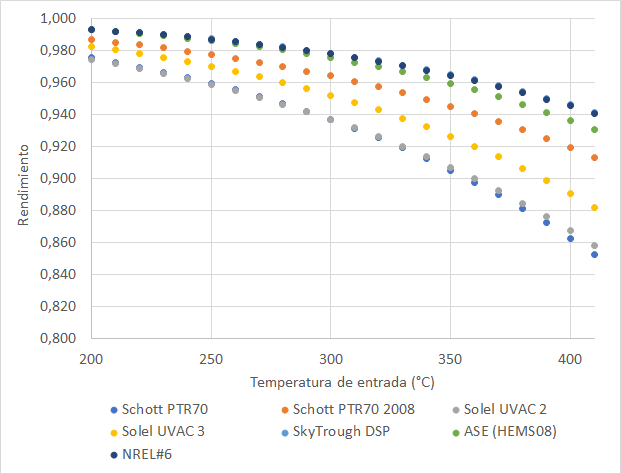
\includegraphics[width=0.9\linewidth]{images/rendimiento_temperatura.png}
\caption[Rendimiento térmico en función de la temperatura de entrada del HTF para diferentes modelos de HCE]{Rendimiento térmico en función de la temperatura de entrada del HTF para diferentes modelos de HCE. $DNI= 800 W/m^2$, $\dot m$ = 6 kg/s} 
\label{fig:test2a}
\end{figure}

\subsection{Rendimiento del HCE en función del flujo de radiación absorbido, $\dot q''_{abs}$}

El flujo de radiación absorbido, $\dot q''_{abs}$,  también es un factor determinante en el diseño del concentrador solar. Es interesante comprobar que el rendimiento aumenta según lo hace $\dot q''_{abs}$ pero, tal y como se aprecia en la Fig. \ref{fig:rendimiento_qabs}, el Modelo de 4º Orden recoge la presencia de un máximo que no es recogido por los modelos de menos precisos.  En todo caso, este máximo se encuentra para para valores de flujo máximo muy superiores a los que se alcanzan con factores de concentración propios de CCP.

\begin{figure}[H]
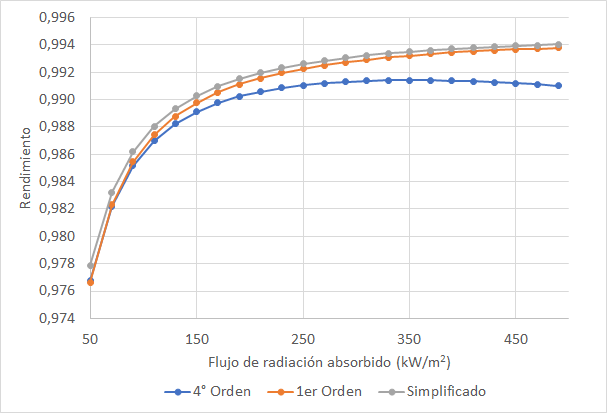
\includegraphics[width=0.9\linewidth]{images/rendimiento_qabs.png}
\caption[Rendimiento térmico en función del flujo de radiación absorbido para diferentes modelos de HCE]{Rendimiento térmico en función del flujo de radiación absorbido para diferentes modelos de HCE. $t_{in}$= 300 ºC, $\dot m$ = 6 kg/s} 
\label{fig:rendimiento_qabs}
\end{figure}

Los valores correspondientes se muestran en la tabla \ref{tab:rendimiento_qabs}.

\begin{longtable}[c]{cccc}
\caption{Rendimiento en función del flujo de radiación absorbido y para cada modelo teórico}
\label{tab:rendimiento_qabs} \\ \hline
$\rule{0pt}{2ex} \dot q''_{abs}$    & 4° Orden & $1^{er}$ Orden & Simplificado \\ \hline
\endfirsthead
\multicolumn{4}{c}%
{{Tabla \thetable\ continúa desde la página anterior}} \\ \hline
$\rule{0pt}{2ex} \dot q''_{abs}$    & 4° Orden & $1^{er}$ Orden & Simplificado \\ \hline
\endhead
50000  & 0,9768 & 0,9766 & 0,9779 \\
70000  & 0,9822 & 0,9823 & 0,9832 \\
90000  & 0,9852 & 0,9854 & 0,9862 \\
110000 & 0,9870 & 0,9874 & 0,9881 \\
130000 & 0,9882 & 0,9888 & 0,9893 \\
150000 & 0,9891 & 0,9898 & 0,9903 \\
170000 & 0,9898 & 0,9905 & 0,9910 \\
190000 & 0,9902 & 0,9911 & 0,9915 \\
210000 & 0,9906 & 0,9916 & 0,9920 \\
230000 & 0,9908 & 0,9919 & 0,9923 \\
250000 & 0,9910 & 0,9923 & 0,9926 \\
270000 & 0,9912 & 0,9925 & 0,9929 \\
290000 & 0,9913 & 0,9927 & 0,9931 \\
310000 & 0,9914 & 0,9929 & 0,9932 \\
330000 & 0,9914 & 0,9931 & 0,9934 \\
350000 & 0,9914 & 0,9932 & 0,9935 \\
370000 & 0,9914 & 0,9933 & 0,9936 \\
390000 & 0,9914 & 0,9934 & 0,9937 \\
410000 & 0,9913 & 0,9935 & 0,9938 \\
430000 & 0,9913 & 0,9936 & 0,9939 \\
450000 & 0,9912 & 0,9937 & 0,9939 \\
470000 & 0,9911 & 0,9937 & 0,9940 \\
490000 & 0,9910 & 0,9938 & 0,9940 \\
\end{longtable}


\subsection{Simulación con los diferentes modelos teóricos}

Comparamos ahora el resultado de simular con los tres modelos: modelo de 4º Orden, modelo de $1^{er}$ Orden y modelo Simplificado. En las siguientes figuras podemos comparar los resultados de temperatura, caudal, rendimiento y potencia térmica de la configuración de campo solar empleada en el apartado \ref{configuracion-simulaciones} para un día del año (se ha tomado el día 2 de marzo por tener buenas condiciones de radiación y estabilidad). 

\begin{longtable}[c]{ccccccc}
\caption[Temperaturas obtenidas en la simulación con cada modelo teórico en un día de condiciones estables]{Temperaturas obtenidas en la simulación con cada modelo teórico. Datos del día 2/3/2007. Condiciones estables y buena radiación}
\label{tab:temperaturas_modelos} \\ \hline
Hora &
\parbox{4em}{\centering DNI \\ $(W/m^2)$} &
\parbox{4em}{\centering \rule{0pt}{2ex} $T_{in}$ \\ $(^\circ C)$} &
\parbox{4em}{\centering \rule{0pt}{2ex} $T_{out}$  (SAM) \\ $(^\circ C)$} &
\parbox{4em}{\centering \rule{0pt}{2ex} $T_{out}$ ($4^o Ord.$) \\ $(^\circ C)$} &
\parbox{4em}{\centering \rule{0pt}{2ex} $T_{out}$  ($1^{er} Ord.$) \\ $(^\circ C)$} &
\parbox{4em}{\centering \rule{0pt}{2ex} $T_{out}$ (Simplif.) \\  $(^\circ C)$}  \\ \hline
\endfirsthead
\multicolumn{7}{c}%
{{Tabla \thetable\ continúa desde la página anterior}} \\ \hline
Hora &
\parbox{4em}{\centering DNI \\ $(W/m^2)$} &
\parbox{4em}{\centering \rule{0pt}{2ex} $T_{in}$ \\ $(^\circ C)$} &
\parbox{4em}{\centering \rule{0pt}{2ex} $T_{out}$  (SAM) \\ $(^\circ C)$} &
\parbox{4em}{\centering \rule{0pt}{2ex} $T_{out}$ ($4^o Ord.$) \\ $(^\circ C)$} &
\parbox{4em}{\centering \rule{0pt}{2ex} $T_{out}$  ($1^{er} Ord.$) \\ $(^\circ C)$} &
\parbox{4em}{\centering \rule{0pt}{2ex} $T_{out}$ (Simplif.) \\  $(^\circ C)$}  \\ \hline
\endhead
0:00  & 0   & 277 & 266 & 266 & 266 & 261 \\ 
1:00  & 0   & 273 & 262 & 262 & 262 & 258 \\
2:00  & 0   & 269 & 259 & 258 & 258 & 254 \\
3:00  & 0   & 265 & 255 & 255 & 255 & 251 \\
4:00  & 0   & 262 & 252 & 251 & 251 & 248 \\
5:00  & 0   & 258 & 249 & 248 & 248 & 245 \\
6:00  & 0   & 255 & 246 & 245 & 245 & 242 \\
7:00  & 234 & 252 & 263 & 243 & 243 & 240 \\
8:00  & 596 & 272 & 377 & 393 & 393 & 393 \\
9:00  & 724 & 292 & 392 & 393 & 393 & 393 \\
10:00 & 806 & 293 & 393 & 393 & 393 & 393 \\
11:00 & 859 & 293 & 393 & 393 & 393 & 393 \\
12:00 & 876 & 293 & 393 & 393 & 393 & 393 \\
13:00 & 867 & 293 & 393 & 393 & 393 & 393 \\
14:00 & 846 & 293 & 393 & 393 & 393 & 393 \\
15:00 & 781 & 293 & 393 & 393 & 393 & 393 \\
16:00 & 663 & 293 & 393 & 393 & 393 & 393 \\
17:00 & 420 & 293 & 313 & 281 & 281 & 275 \\
18:00 & 1   & 293 & 284 & 281 & 281 & 275 \\
19:00 & 0   & 298 & 282 & 285 & 285 & 280 \\
20:00 & 0   & 298 & 284 & 285 & 285 & 279 \\
21:00 & 0   & 293 & 281 & 281 & 281 & 276 \\
22:00 & 0   & 289 & 277 & 277 & 277 & 272 \\
23:00 & 0   & 284 & 273 & 273 & 273 & 268 \\
\end{longtable}

El resultado gráfico de este test puede verse en la figura Fig.\ref{fig:temperaturas_modelos}, donde se aprecia que todos los modelos encuentran soluciones similares en la simulación. El resultado era de esperar pues las temperaturas de trabajo, inferiores a 400 ºC, están dentro del rango de validez de aplicación de todos los modelos. Otra vez los resultados son muy parecidos a los obtenidos con SAM.

\begin{figure}[H]
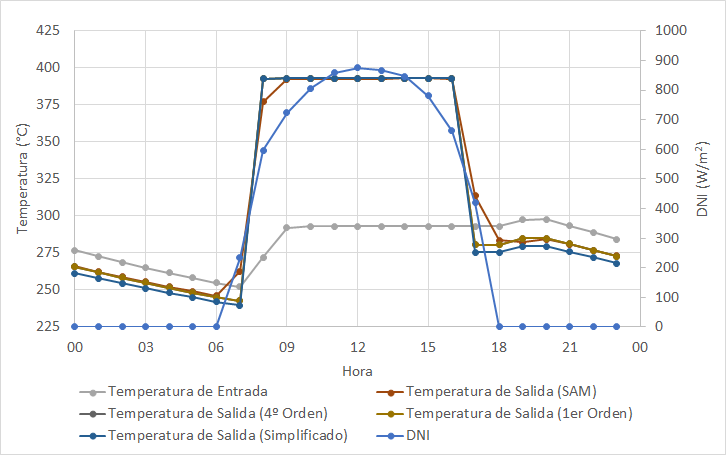
\includegraphics[width=0.9\linewidth]{images/temperaturas_modelos.png}
\caption[Temperaturas de salida obtenidas con los tres modelos]{Temperaturas de salida obtenidas con los tres modelos. Simulación con los datos del día 2/3/2007.} 
\label{fig:temperaturas_modelos}
\end{figure}

En el caso de los caudales y la potencia térmica  los resultados son similares, tal y como se aprecia en las figuras \ref{fig:caudales_modelos} y \ref{fig:potencias_modelos} respectivamente. Los valores numéricos se muestran en las tablas \ref{tab:caudales_modelos} y  \ref{tab:potencias_modelos}.

\begin{figure}[H]
\caption[Caudales de salida obtenidos con los tres modelos en un día de condiciones estables]{Caudales de salida obtenidos con los tres modelos. Datos del día 2/3/2007. Condiciones estables y buena radiación} 
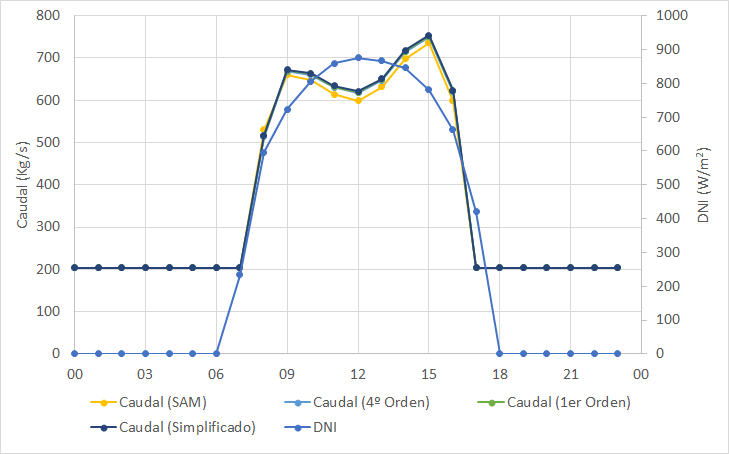
\includegraphics[width=0.9\linewidth]{images/caudales_modelos.png}
\label{fig:caudales_modelos}
\end{figure}

\begin{figure}[H]
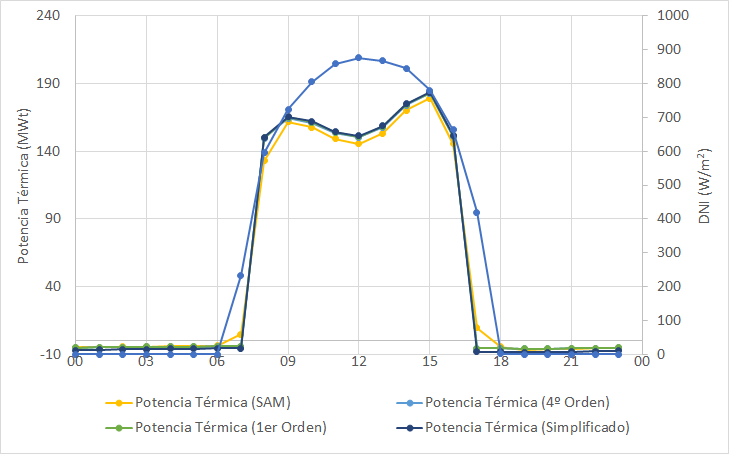
\includegraphics[width=0.9\linewidth]{images/potencias_modelos.png}
\caption[Potencia térmica obtenida con cada uno de los tres modelos en un día de condiciones estables]{Potencia térmica obtenida con cada uno de los tres modelos. Datos del día 2/3/2007. Condiciones estables y buena radiación} 
\label{fig:potencias_modelos}
\end{figure}

\begin{longtable}[c]{cccccc}
\caption[Caudales obtenidos en la simulación para cada modelo en un día de condiciones estables]{Caudales obtenidos en la simulación para cada modelo.  Datos del día 2/3/2007. Condiciones estables y buena radiación}
\label{tab:caudales_modelos} \\ \hline
Hora &
\parbox{4em}{\centering DNI \\ $(W/m^2)$} &
\parbox{4em}{\centering \rule{0pt}{2ex}Caudal  (SAM) \\ $(kg/s)$} &
\parbox{4em}{\centering \rule{0pt}{2ex}Caudal ($4^o Ord.$) \\ $(kg/s)$} &
\parbox{4em}{\centering \rule{0pt}{2ex}Caudal  ($1^{er} Ord.$) \\ $(kg/s)$} &
\parbox{4em}{\centering \rule{0pt}{2ex}Caudal (Simplif.) \\  $(kg/s)$}  \\ \hline
\endfirsthead
\multicolumn{6}{c}%
{{Tabla \thetable\ continúa desde la página anterior}} \\ \hline
Hora &
\parbox{4em}{\centering DNI \\ $(W/m^2)$} &
\parbox{4em}{\centering \rule{0pt}{2ex}Caudal  (SAM) \\ $(kg/s)$} &
\parbox{4em}{\centering \rule{0pt}{2ex}Caudal ($4^o Ord.$) \\ $(kg/s)$} &
\parbox{4em}{\centering \rule{0pt}{2ex}Caudal  ($1^{er} Ord.$) \\ $(kg/s)$} &
\parbox{4em}{\centering \rule{0pt}{2ex}Caudal (Simplif.) \\  $(kg/s)$}  \\ \hline \\
\endhead
0:00  & 0   & 204          & 204               & 204                & 204                   \\ 
1:00  & 0   & 204          & 204               & 204                & 204                   \\ 
2:00  & 0   & 204          & 204               & 204                & 204                   \\ 
3:00  & 0   & 204          & 204               & 204                & 204                   \\ 
4:00  & 0   & 204          & 204               & 204                & 204                   \\ 
5:00  & 0   & 204          & 204               & 204                & 204                   \\ 
6:00  & 0   & 204          & 204               & 204                & 204                   \\ 
7:00  & 234 & 204          & 204               & 204                & 204                   \\ 
8:00  & 596 & 530          & 514               & 516                & 518                   \\ 
9:00  & 724 & 660          & 669               & 670                & 672                   \\ 
10:00 & 806 & 648          & 661               & 663                & 664                   \\ 
11:00 & 859 & 614          & 630               & 632                & 634                   \\ 
12:00 & 876 & 599          & 617               & 619                & 621                   \\ 
13:00 & 867 & 632          & 648               & 650                & 651                   \\ 
14:00 & 846 & 699          & 714               & 716                & 718                   \\ 
15:00 & 781 & 736          & 750               & 752                & 753                   \\ 
16:00 & 663 & 599          & 620               & 622                & 624                   \\ 
17:00 & 420 & 204          & 204               & 204                & 204                   \\ 
18:00 & 1   & 204          & 204               & 204                & 204                   \\ 
19:00 & 0   & 204          & 204               & 204                & 204                   \\ 
20:00 & 0   & 204          & 204               & 204                & 204                   \\ 
21:00 & 0   & 204          & 204               & 204                & 204                   \\ 
22:00 & 0   & 204          & 204               & 204                & 204                   \\ 
23:00 & 0   & 204          & 204               & 204                & 204                   \\
\end{longtable}

\begin{longtable}[c]{cccccc}
\caption[Potencia térmica calculada en la simulación de cada modelo en un día de condiciones estables]{Potencia térmica calculada en la simulación de cada modelo.  Datos del día 2/3/2007. Condiciones estables y buena radiación}
\label{tab:potencias_modelos} \\ \hline
Hora &
\parbox{4em}{\centering DNI \\ $(W/m^2)$} &
\parbox{4em}{\centering \rule{0pt}{2ex} $P_{th}$  (SAM) \\  $(MWt)$} &
\parbox{4em}{\centering \rule{0pt}{2ex} $P_{th}$ ($4^o Ord.$) \\  $(MWt)$} &
\parbox{4em}{\centering \rule{0pt}{2ex} $P_{th}$  ($1^{er} Ord.$) \\  $(MWt)$} &
\parbox{4em}{\centering \rule{0pt}{2ex} $P_{th}$ (Simplif.) \\   $(MWt)$}  \\ \hline
\endfirsthead
\multicolumn{6}{c}
{{Tabla \thetable\ continúa desde la página anterior}} \\ \hline
Hora &
\parbox{4em}{\centering DNI \\ $(W/m^2)$} &
\parbox{4em}{\centering \rule{0pt}{2ex} $P_{th}$  (SAM) \\  $(MWt)$} &
\parbox{4em}{\centering \rule{0pt}{2ex} $P_{th}$ ($4^o Ord.$) \\  $(MWt)$} &
\parbox{4em}{\centering \rule{0pt}{2ex} $P_{th}$  ($1^{er} Ord.$) \\  $(MWt)$} &
\parbox{4em}{\centering \rule{0pt}{2ex} $P_{th}$ (Simplif.) \\   $(MWt)$}  \\ \hline
\endhead
0:00  & 0   & -4,9  & -5,0  & -5,0  & -6,9  \\
1:00  & 0   & -4,7  & -4,9  & -4,9  & -6,7  \\
2:00  & 0   & -4,5  & -4,8  & -4,8  & -6,5  \\
3:00  & 0   & -4,4  & -4,6  & -4,6  & -6,3  \\
4:00  & 0   & -4,2  & -4,5  & -4,5  & -6,0  \\
5:00  & 0   & -4,1  & -4,4  & -4,4  & -5,9  \\
6:00  & 0   & -3,9  & -4,3  & -4,3  & -5,7  \\
7:00  & 234 & 4,7   & -4,2  & -4,2  & -5,6  \\
8:00  & 596 & 133,1 & 149,5 & 150,1 & 150,5 \\
9:00  & 724 & 161,6 & 164,6 & 165,0 & 165,4 \\
10:00 & 806 & 157,7 & 161,2 & 161,6 & 162,1 \\
11:00 & 859 & 149,2 & 153,6 & 154,1 & 154,5 \\
12:00 & 876 & 145,5 & 150,5 & 150,9 & 151,3 \\
13:00 & 867 & 153,4 & 157,9 & 158,3 & 158,8 \\
14:00 & 846 & 170,2 & 174,2 & 174,6 & 175,0 \\
15:00 & 781 & 179,3 & 182,7 & 183,2 & 183,6 \\
16:00 & 663 & 145,6 & 151,1 & 151,6 & 152,0 \\
17:00 & 420 & 9,7   & -5,7  & -5,7  & -8,2  \\
18:00 & 1   & -4,4  & -5,7  & -5,7  & -8,1  \\
19:00 & 0   & -7,1  & -5,9  & -5,9  & -8,4  \\
20:00 & 0   & -6,3  & -5,9  & -5,9  & -8,4  \\
21:00 & 0   & -5,8  & -5,7  & -5,7  & -8,1  \\
22:00 & 0   & -5,5  & -5,5  & -5,5  & -7,8  \\
23:00 & 0   & -5,3  & -5,4  & -5,4  & -7,5 
\end{longtable}


\subsection{Simulación cambiando el tamaño de la malla de integración}
\label{mallaintegracion}

En el caso de tener que realizar un gran número de simulaciones, el tiempo de cálculo puede ser un factor limitante. Una forma de reducirlo es aumentando el tamaño de la malla de integración. Esto es equivalente a considerar un HCE de tamaño mayor al real, con lo que el número de cálculos por lazo se reduce. Realizamos una simulación con cada modelo teórico en la que calculamos el rendimiento térmico de un lazo completo variando el tamaño de malla de integración.  

En las figuras  \ref{fig:malla0405} a \ref{fig:malla14580} se aprecia una mayor divergencia en el rendimiento calculado por cada modelo a medida que aumenta el tamaño de malla. Las diferencias son mayores para valores más altos de DNI. Como conclusión, podemos aceptar tamaños de malla de no más de 100 m para el Modelo de 4º Orden. Para el Modelo de $1^{er}$ Orden y el Modelo Simplificado vemos que una malla de unos 50 m ya empieza a mostrar diferencias apreciables respecto al modelo de 4º Orden.

\begin{figure}[H]
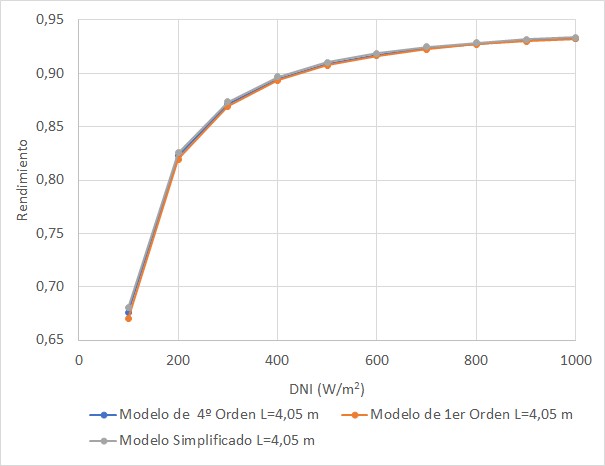
\includegraphics[width=0.87\linewidth]{images/malla0405.png}
\caption{Rendimiento calculado con cada modelo para un tamaño de malla de integración de 4,05 m} 
\label{fig:malla0405}
\end{figure}

\begin{figure}[H]
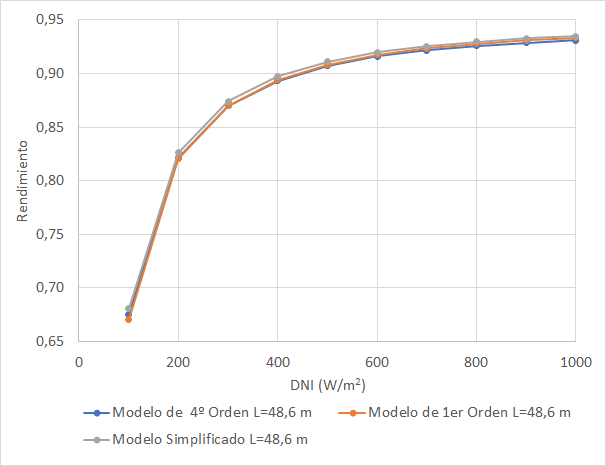
\includegraphics[width=0.87\linewidth]{images/malla4860.png}
\caption{Rendimiento calculado con cada modelo para un tamaño de malla de integración de 48,60 m} 
\label{fig:malla4860}
\end{figure}

\begin{figure}[H]
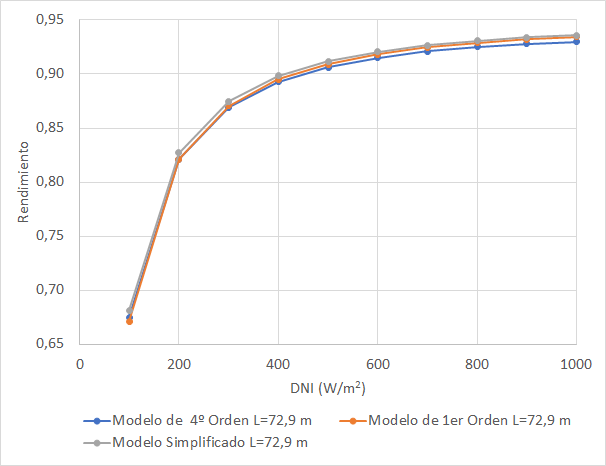
\includegraphics[width=0.87\linewidth]{images/malla7290.png}
\caption{Rendimiento calculado con cada modelo para un tamaño de malla de integración de 72,90 m} 
\label{fig:malla7290}
\end{figure}

\begin{figure}[H]
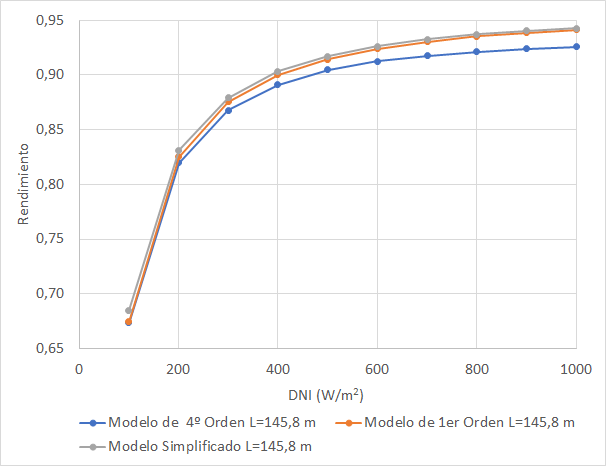
\includegraphics[width=0.87\linewidth]{images/malla14580.png}
\caption{Rendimiento calculado con cada modelo para un tamaño de malla de integración de 145,80 m} 
\label{fig:malla14580}
\end{figure}

En la Fig.\ref{fig:malla_variable_DNI_800} hemos representado el rendimiento, calculado para unas determinadas condiciones de operación, en función del tamaño de malla (el eje de abscisas tiene una escala $log_2$). Según aumenta el tamaño de malla se produce una ligera variación en el rendimiento calculado que comienza a crecer más rápidamente alrededor de 100 m, manteniéndose por debajo del 1\% mientras no se supere ese límite de tamaño de malla de integración. 

\begin{figure}[H]
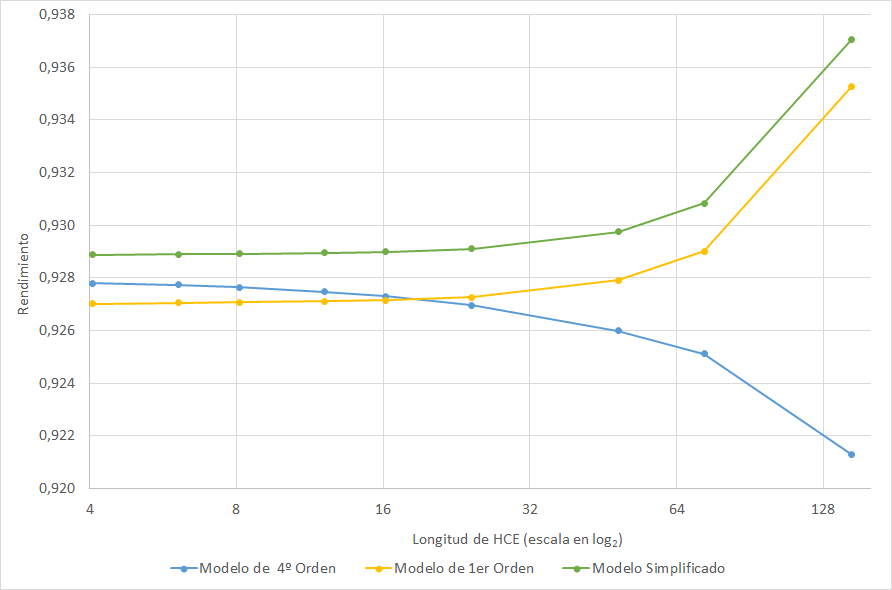
\includegraphics[width=0.9\linewidth]{images/malla_variable_DNI_800.png}
\caption[Rendimiento calculado para diferentes tamaños de malla de integración]{Rendimiento calculado para diferentes tamaños de malla de integración. $DNI=800 W/m^2$, $T_{in}=300 ^\circ C$, $\dot m = 6 kg/s$} 
\label{fig:malla_variable_DNI_800}
\end{figure}

En la serie de figuras \ref{fig:desviacionmodel4} a \ref{fig:desviacionmodelsimplificado} podemos ver cómo aumenta la desviación, para cada modelo y en función de $DNI$, entre el rendimiento calculado para un determinado tamaño de malla y el rendimiento calculado con una malla de 4,05 m (tamaño real del HCE).

\begin{figure}[H]
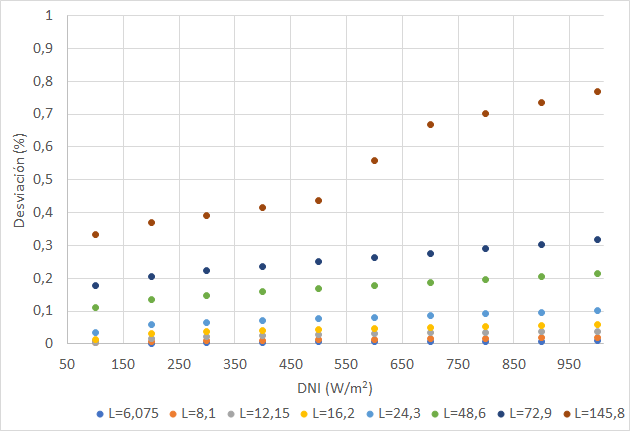
\includegraphics[width=0.9\linewidth]{images/desviacionmodel4malla.png}
\caption[Desviación, para simulaciones con el Modelo de 4º Orden, según diferentes tamaños de malla]{Desviación, para simulaciones con el Modelo de 4º Orden, según diferentes tamaños de malla. Los valores muestran la desviación, en tanto por ciento, respecto a la simulación con una malla de 4,05 m. $T_{in}=300 ^\circ C$, $\dot m = 6 kg/s$} 
\label{fig:desviacionmodel4}
\end{figure}

\begin{figure}[H]
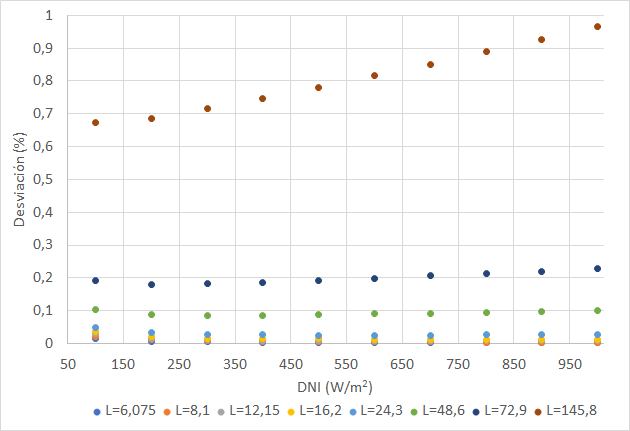
\includegraphics[width=0.9\linewidth]{images/desviacionmodel1malla.png}
\caption[Desviación, para simulaciones con el Modelo de $1^{er}$ Orden, según diferentes tamaños de malla]{Desviación, para simulaciones con el Modelo de $1^{er}$ Orden, según diferentes tamaños de malla. Los valores muestran la desviación, en tanto por ciento, respecto a la simulación con una malla de 4,05 m. $T_{in}=300 ^\circ C$, $\dot m = 6 kg/s$} 
\label{fig:desviacionmodel1}
\end{figure}

\begin{figure}[H]
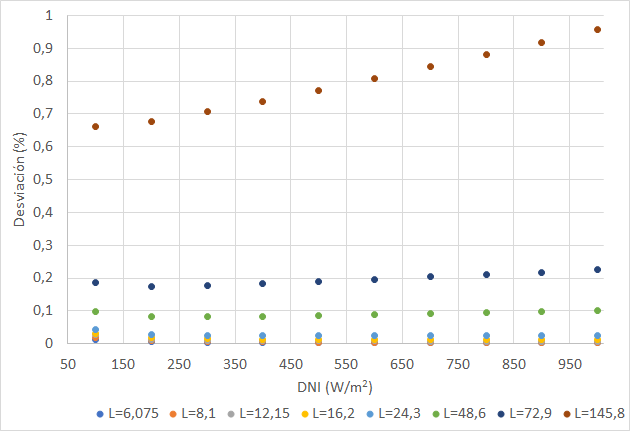
\includegraphics[width=0.9\linewidth]{images/desviacionmodelsimplificadomalla.png}
\caption[Desviación, para simulaciones con el Modelo de Simplificado, según diferentes tamaños de malla]{Desviación, para simulaciones con el Modelo de Simplificado, según diferentes tamaños de malla. Los valores muestran la desviación, en tanto por ciento, respecto a la simulación con una malla de 4,05 m. $T_{in}=300 ^\circ C$, $\dot m = 6 kg/s$} 
\label{fig:desviacionmodelsimplificado}
\end{figure}


\section{Análisis de los datos de generación de una planta solar termoeléctrica real}
\label{descripcion-central}

Finalmente emplearemos nuestro programa de simulación en un análisis del estado del campo solar de una planta termosolar real. Puesto que la simulación de sistemas externos al campo solar queda fuera de nuestro alcance, nos centraremos en los datos referentes al campo solar. En concreto, contrastaremos  qué potencia térmica se extrae del campo, independientemente de las causas operativas que condicionasen el funcionamiento de la planta en cada momento. Realizaremos la simulación a partir de datos reales (meteorológicos y de generación) de una central termosolar, comparando el salto térmico real con el simulado. 

La configuración de campo solar que se va a utilizar a lo largo de las siguientes simulaciones está basada en las plantas termosolares Aste 1A y 1B, que se encuentran situadas en el término municipal de Alcázar de San Juan, provincia de Ciudad Real. Sus coordenadas geográficas son (39,1°N 3,16°W) y la altitud es de 651 m sobre el nivel del mar.

\begin{figure}[H]
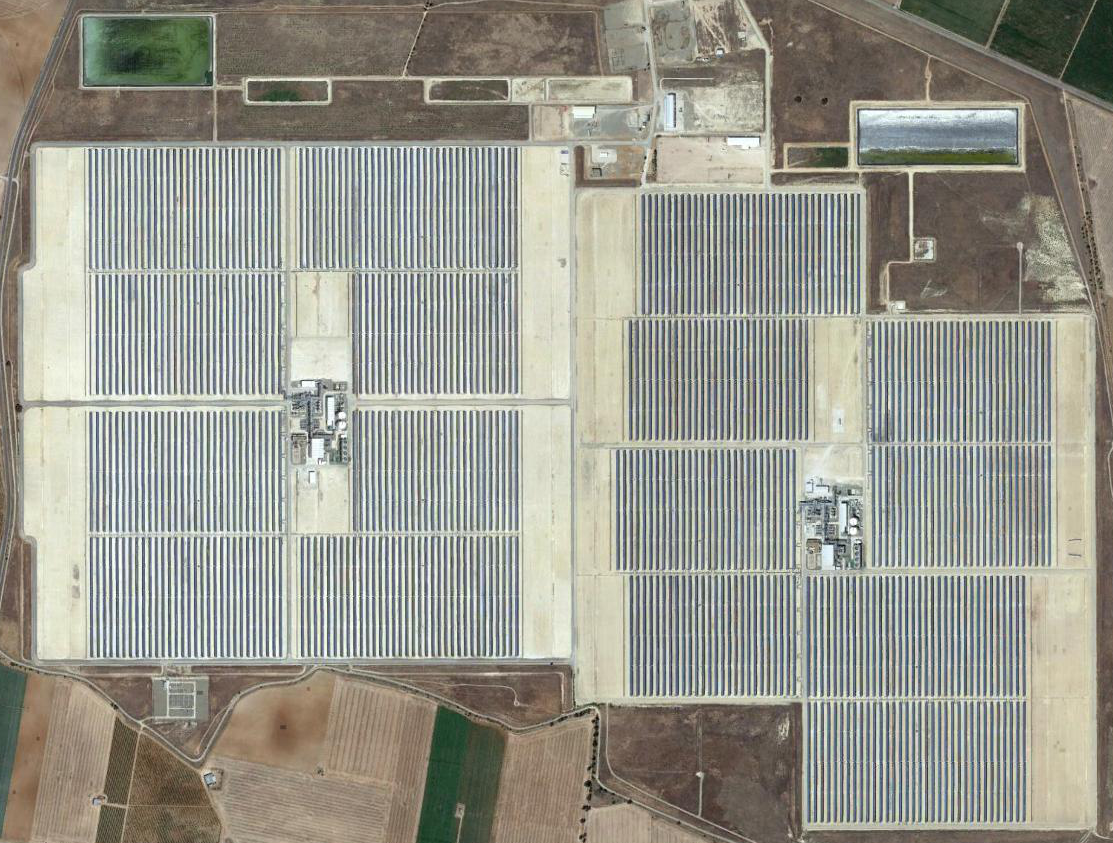
\includegraphics[width=0.9\linewidth]{images/fotoAstes.png}
\caption[Vista aérea de las centrales Aste 1A y Aste 1B]{Centrales Termosolares Aste 1A (izq.) y Aste 1B (der.) Fuente: Google Earth} 
\label{fig:astes}
\end{figure}

La potencia eléctrica nominal de cada una de ellas es de 49,9 MW. El proyecto inicial consideraba que las plantas contarían con almacenamiento térmico, el cual se construiría durante una segunda fase que finalmente no se llegó a ejecutar, por lo que en la actualidad solo existe generación durante las horas de sol. Se emplearán los datos de Aste 1B, cuya configuración es la siguiente:

El campo solar cuenta con 120 lazos distribuidos de manera irregular en 4 subcampos. La  distancia de separación entre lazos es de 16,25 m. 

\begin{itemize}[itemsep=2pt,parsep=2pt]
\item
  Subcampo NO, 31 lazos.
\item
  Subcampo NE, 28 lazos.
\item
  Subcampo SO, 27 lazos.
\item
  Subcampo SE, 34 lazos.
\end{itemize}

Todos los lazos son idénticos, contando con 4 SCAs cada uno en una configuración tipo \(U\). El eje de seguimiento perfectamente plano se encuentra alineado en dirección N-S. Cada SCA cuenta con un total de 336 espejos de vidrio fabricados por Flabeg. 

La reflectividad de los espejos puede obtenerse a partir de los registros de mantenimiento de ese año. Llegados a este punto encontramos cierta anomalía en los valores recopilados, tal y como puede apreciarse en la \ref{fig:reflectividad}. Se observa cómo durante los meses de junio y julio el valor de la reflectividad promedio comienza a caer drásticamente hasta valores ligeramente inferiores al 60\%. Los valores van mejorando posteriormente, durante el mes de agosto, hasta alcanzar valores normales a partir de septiembre.

\begin{figure}[H]
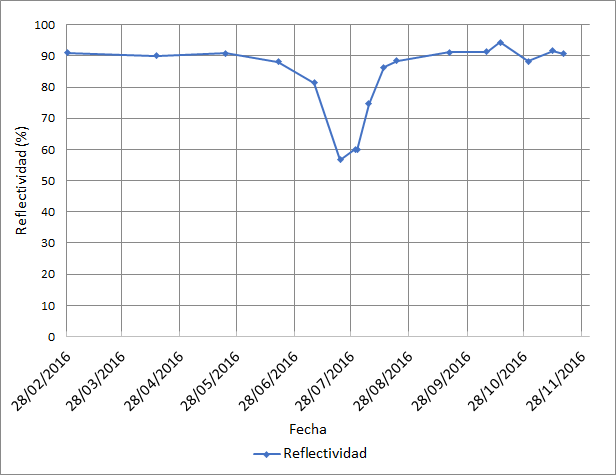
\includegraphics[width=0.9\linewidth]{images/reflectividad.png}
\caption[Reflectividad registrada durante el mantenimiento]{Reflectividad registrada durante el mantenimiento. Fuente: CST Aste 1B} 
\label{fig:reflectividad}
\end{figure}

El origen de este comportamiento está en que durante ese periodo se paralizó la actividad de limpieza de espejos (por causas indeterminadas). Una vez que se reanuda el mantenimiento y limpieza del campo solar, los valores de reflectividad vuelven a su valor habitual, alrededor del 90\%. Debe tenerse en cuenta que la limpieza de espejos de todo el campo puede requerir varias semanas para un equipo de mantenimiento compuesto por un solo camión de agua presurizada apoyado por dos operarios con un ritmo normal de limpieza de unos 8 a 10 lazos cada noche. Esta contingencia no afectó a la generación eléctrica de la planta por estar el campo solar muy sobredimensionado.

Respecto al estado de los tubos HCE, consideraremos que se encuentran en buen estado de vacío. Los recuentos anuales efectuados en planta indican que tras 4 años de operación apenas se contabiliza una media de un HCE sin vacío por cada lazo y el número de HCE sin envolvente de vidrio es despreciable (apenas una veintena de unidades de un total de 17280 unidades en todo el campo).

El fluido de trabajo es \emph{Dowtherm-A}, cuyas propiedades también se han descrito en el apartado \ref{subclases-fluid}.

Los datos meteorológicos son los recogidos a lo largo de 2016 por las tres estaciones meteorológicas con las que cuenta la planta. Al tener por triplicado las medidas de cada variable se adopta el criterio de seleccionar la mediana de las tres y no el valor medio. Esta selección la realiza el sistema de control de planta en cada momento y con este criterio se persigue conseguir una mayor robustez del sistema, pues si una estación presenta valores muy desviados de las otras dos podría darse el caso de que el valor medio estuviese muy alejado del valor  verdadero. Cuando por avería o fallo de comunicación se carece de los datos de alguna estación sí se suele adoptar el criterio de seleccionar el valor medio de las dos restantes.

Los datos de las figuras \ref{fig:temperatura_1b} a \ref{fig:caudal_1b} muestran el comportamiento de la planta real para un día de buena radiación y condiciones estables. Puesto que la planta no dispone de almacenamiento energético, los efectos de las inercias de arranque y parada se aprecian claramente a primera y última hora del día, así como en los altibajos de radiación en los días inestables. En esta planta, el control de caudal lo realiza manualmente el operador de sala en base a las diferentes limitaciones que el diseño de planta impone. Especialmente importantes son los gradientes de calentamiento o, más apropiadamente, las rampas de calentamiento y enfriamiento que los fabricantes de los equipos recomiendan, como es el caso de la turbina, trenes de generación, bombas principales de HTF o los propios HCEs. También existe una inercia asociada al calentamiento de tuberías y tanques de expansión y rebose.  La masa total de HTF en la planta ronda las 1300 toneladas. 

En nuestra simulación, la temperatura de salida consignada se alcanza por la mañana más rápidamente de lo que lo hace realmente, al no incluir nuestro modelo ninguna inercia térmica para el calentamiento de todo el sistema. Algo parecido ocurre a la salida, donde el \''enfriamiento\'' de la planta se produce más lentamente en la realidad que en la simulación, \ref{fig:temperatura_1b}.

\begin{figure}[H]
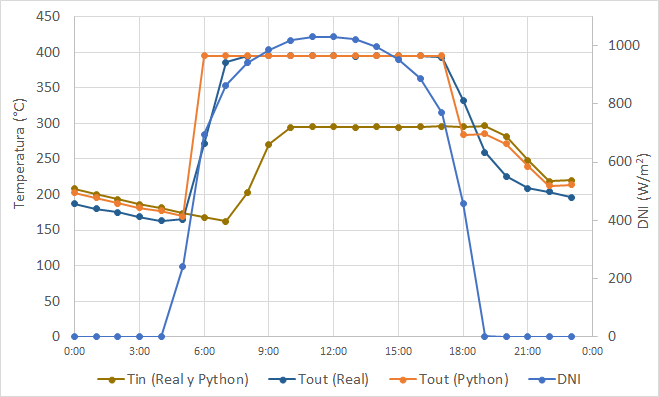
\includegraphics[width=0.9\linewidth]{images/temperatura_aste1b_01052016.png}
\caption[Temperaturas de operación reales y simuladas en un día de condiciones estables]{Temperaturas de operación reales y simuladas para el día 1/5/2016. Condiciones estables y buena radiación} 
\label{fig:temperatura_1b}
\end{figure}

En la  Fig.\ref{fig:potencia_1b} vemos el pico de potencia térmica que realmente se extrae a primera hora de la mañana con el fin de calentar el sistema. En la simulación, esa potencia crece hasta el máximo posible y después se aplana pues, tal y como hemos ido explicando a lo largo de este trabajo, nuestro código simula la operación para un sistema que pudiese extraer toda la energía disponible del campo solar. 

\begin{figure}[H]
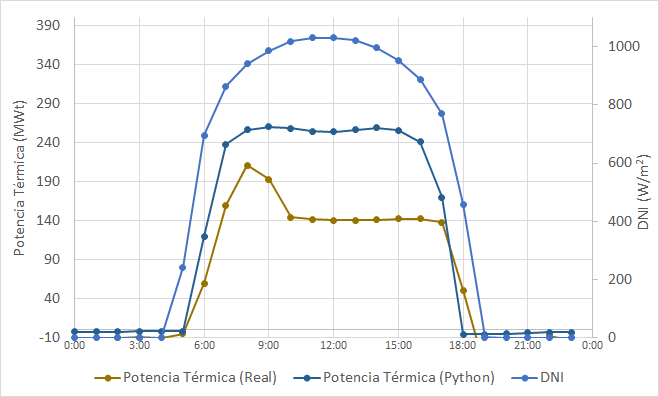
\includegraphics[width=0.9\linewidth]{images/potencia_aste1b_01052016.png}
\caption[Potencia térmica real y simulada en un día de condiciones estables]{Potencia térmica real y simulada para el día 1/5/2016. Condiciones estables y buena radiación} 
\label{fig:potencia_1b}
\end{figure}

Pero en la planta real, al no disponer de almacenamiento térmico, una vez que se dispone de suficiente potencia térmica para suministrar al bloque de potencia, el campo debe empezar a limitarse. Es por este motivo por el que vemos en la Fig.\ref{fig:caudal_1b} que el caudal simulado durante las  horas centrales del día es mucho mayor que el real. 

\begin{figure}[H]
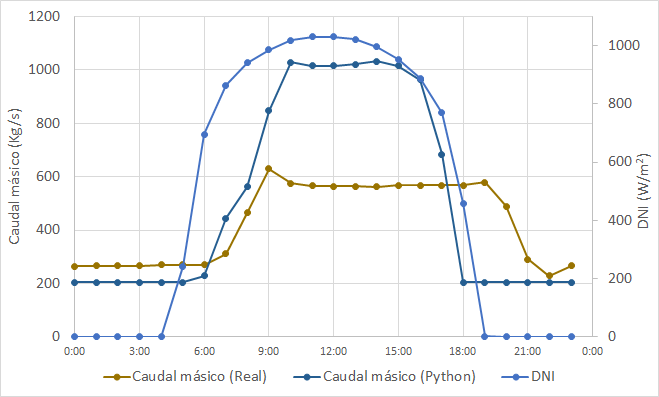
\includegraphics[width=0.9\linewidth]{images/caudal_aste1b_01052016.png}
\caption[Caudal real y simulado en un día de condiciones estables]{Caudal real y simulado para el día 1/5/2016. Condiciones estables y buena radiación} 
\label{fig:caudal_1b}
\end{figure}

Aprovecharemos los datos ofrecidos por nuestro código de simulación para estimar el exceso de energía disponible y el rendimiento global del bloque de potencia y de la planta. No pretendemos alcanzar mucha precisión ya que partimos de datos que en algunos casos pueden contener errores de lectura de instrumentos y que no han sido obtenidos de una forma totalmente controlada. Además, se incluyen datos registrados en condiciones muy diferentes de operación, pero no bajo todas las condiciones ni con el mismo peso en el comportamiento global de la planta, por lo que lo se trata de valores promediados entre el conjunto de la muestra de datos.

Para evitar que estos momentos transitorios afecten a nuestros cálculos filtraremos los datos para tener en cuenta solo aquellos momentos en los que las condiciones de generación ya son estables y todo el sistema se encuentra a plena carga. Para ellos seleccionaremos registros en los que la radiación solar directa, DNI, es superior a 700 $W/m^2$, la temperatura de entrada y salida del campo están muy cerca de las nominales ($T_{in}>290 ^\circ C$  y $T_{out}>390 ^\circ C$). 

Si, bajo este filtro, representamos la potencia térmica real y la potencia térmica simulada (o disponible) en función de DNI, obtenemos la representación de la Fig.\ref{fig:potencia_dni}. Vemos claramente como  la potencia real extraída del campo solar se ha \''estancado\'' alrededor de 140 MWt, mientras que la potencia disponible podría llegar a máximos de algo más de 160 MWt. 

\begin{figure}[H]
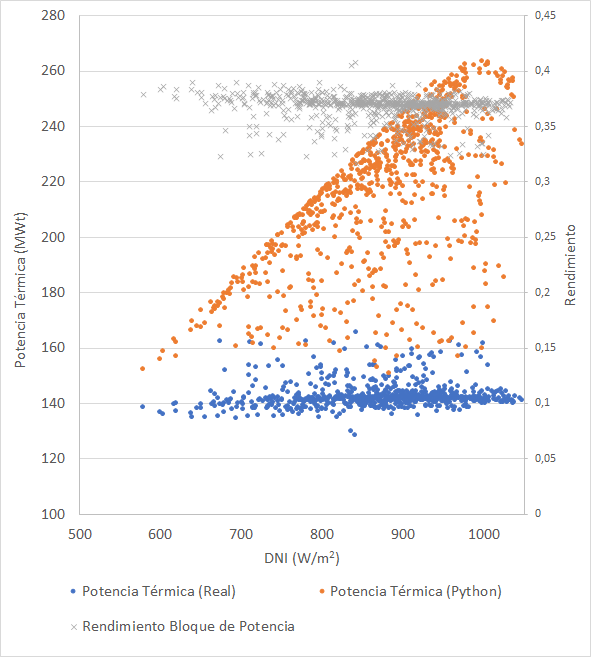
\includegraphics[width=0.9\linewidth]{images/potencia_dni_aste1b.png}
\caption[Potencia térmica real y simulada en función de DNI]{Potencia térmica real y simulada en función de DNI cuando la planta trabaja en condiciones nominales ($T_{in}$>290 ºC, $T_{out}$>390 ºC). En el eje vertical derecho se representa el rendimiento global del bloque de potencia} 
\label{fig:potencia_dni}
\end{figure}

En esa misma figura se ha representado el rendimiento del bloque de potencia entendido como el cociente de la potencia eléctrica bruta de salida del turbogrupo (52,4 MW) entre la potencia térmica extraída del campo solar (140 MWt). Con esta definición, las pérdidas en tuberías y el rendimiento de los trenes de generación de vapor queda incluido dentro de este rendimiento global.  El valor promedio es aproximadamente 0,37 durante condiciones de generación a plena carga.

Nuestro código nos puede servir, llegado a este punto, para cuantificar qué cantidad de energía solar se está desaprovechando debido al sobredimensionado del campo. En condiciones de diseño ($DNI=800 W/m^2$) el campo solar llega a producir 210 MWt de energía térmica, un 50\% más de la demanda necesaria. Este cálculo es compatible con la experiencia de otras plantas en las que no existe almacenamiento, donde es habitual que el campo solar cuente con unos 96 lazos. En plantas de 50 MW con un almacenamiento de unas 6-8 horas el campo solar ronda los 156 lazos.

